\section{introduction}

Serverless computing is another popular trend in the current cloud computing field.
Unlike the traditional IaaS\cite{iaas} or PaaS\cite{paas},
which relies on cloud users to manage virtual machines or configure the capacity and automatic scaling of applications.
Serverless computing delegates all the work of managing virtual machines, execution environments, and software environments to the cloud provider.
Cloud providers makes all the infrastructure management operations transparent to cloud users,
and users only need to focus on writing related functions, which frees users from the trouble of managing servers.
At the same time, serverless computing provides users with a more fine-grained billing model,
which charges based on the actual amount of resources consumed when providing services. Currently serverless computing has been supported by many platforms, including Amazon Lambda\cite{amazon}, IBM Cloud Func\-tion\cite{ibm},
Microsoft Azure Func\-tions\cite{microsoft} and Google Cloud Func\-tions\cite{google}.
At the same time, serverless computing has also developed rapidly in the open source community.
Serverless computing platforms represented by open source projects such as Open\-FaaS\cite{openfaas}, Kube\-less\cite{kubeless}, and K\-native\cite{knative} have received a lot of attention.

Since serverless computing uses an event-driven approach to handle requests,
that is, when each request comes,
a new serverless function is started to process it,
which places high requirements on the efficiency of serverless functions.
The current containerized serverless functions failed to achieve the low startup
latency due to the creation of the isolation environment and the initialization
of the software environment.
The figure\ref{default-proportion} shows the "Execution and Startup/Overall" ratio of five typical serverless
computing applications which are tested on the OpenFaas platform, thoes applications run on different language runtimes.
The experiment shows that on average, the execution latency only accounted for 31\% of overall latency,
at the same time, the overall latency of containerized serverless functions is usually over 100 milliseconds(as shown in the table\ref{overall-latency}),
which obviously cannot meet the high-performance requirements of serverless computing platforms.
\begin{figure}[t]
    \centering
    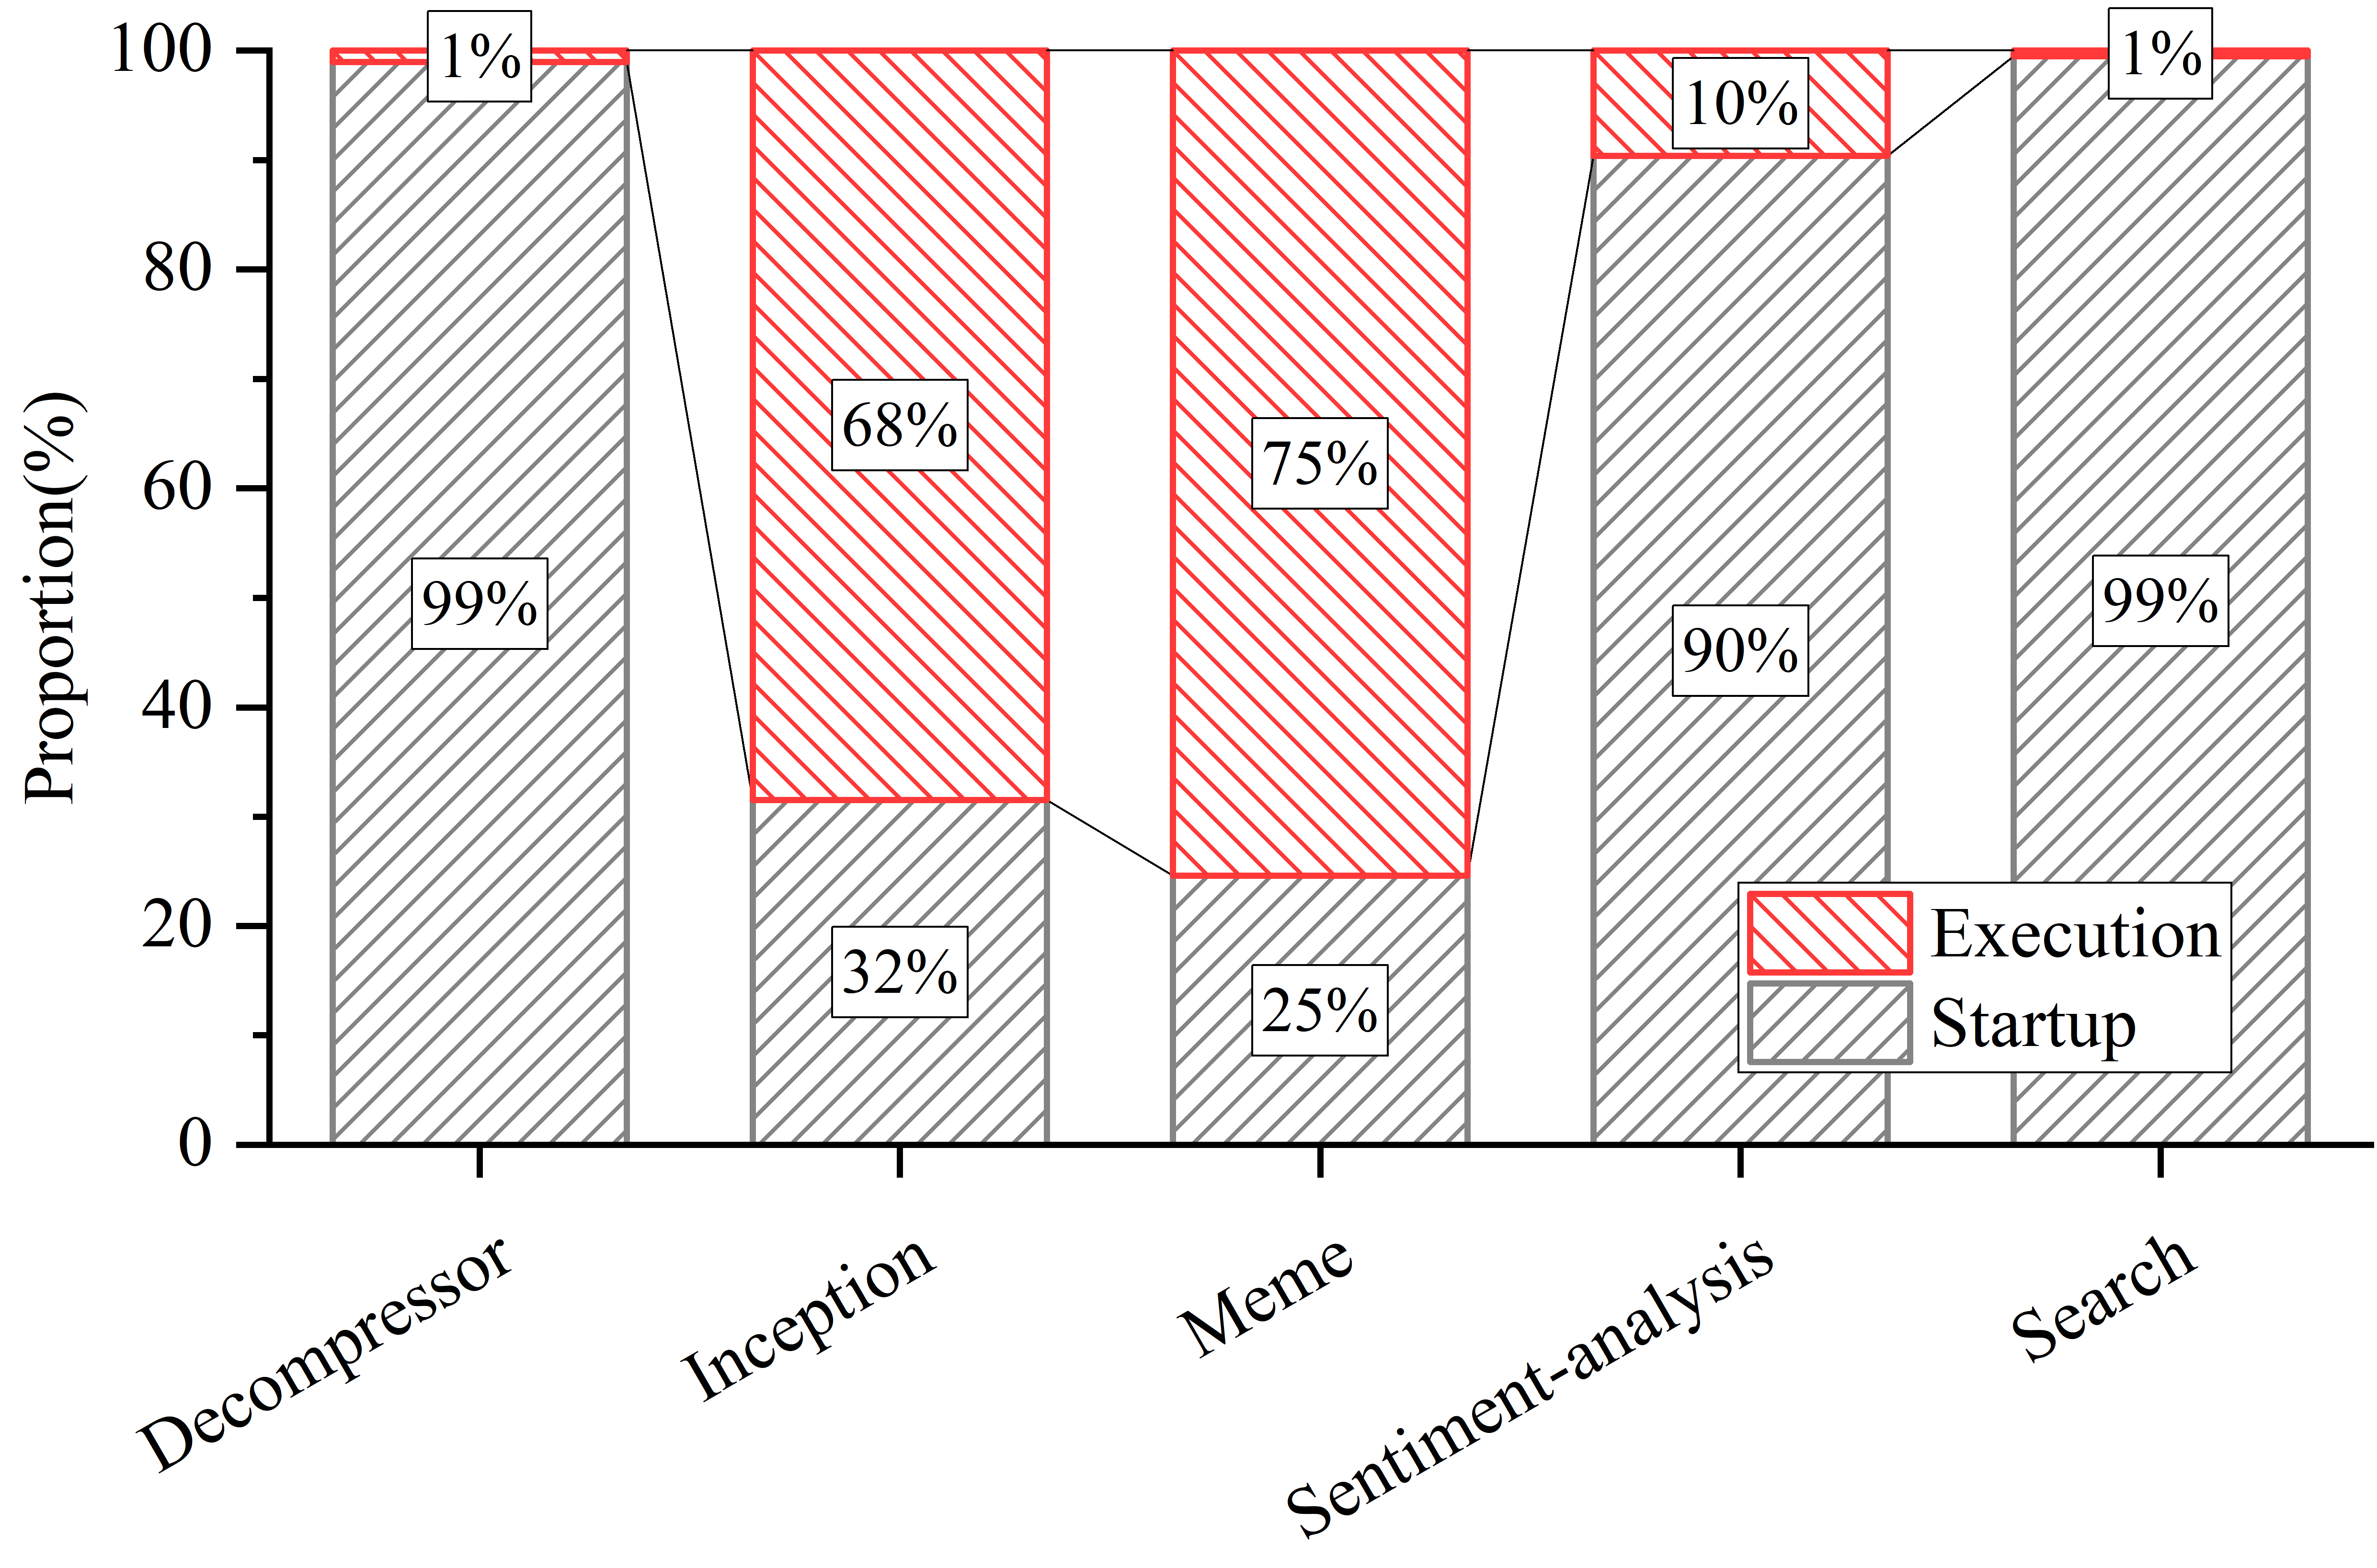
\includegraphics[width=3in]{images/default-proportion.png}
    \caption{Execution(and Startup)/Overall latency ratio of serverless functions.}
    \label{default-proportion}
\end{figure}

\begin{table}[htbp]
    \centering
    \caption{The Overall latency}
    \begin{tabular}{cc}
        \hline
        Type               & Time(ms) \\ \hline
        Decompressor       & 90       \\
        Inception          & 3035     \\
        Meme               & 1228     \\
        Sentiment-analysis & 320      \\
        Search             & 2149     \\ \hline
    \end{tabular}
    \label{overall-latency}
\end{table}

Minimizing the startup latency of serverless functions is critical to improving the user experience of the platform\cite{serverless-user-experience-1,serverless-user-experience-2},
and it is also one of the major challenges facing serverless computing\cite{berkeley-view,serverless-trends}.
Existing solutions reduce the response latency of the serverless computing platform by caching function instances\cite{pool1,pool2} or customizing the virtual environment of functions\cite{firecracker,faasm},
but these solutions cannot effectively reduce the initialization latency of the application.
Subsequent research shows that application initialization accounts for a large part of the function startup latency.


This paper proposes \pname, 
a design that effectively reduces the cold start latency of containerized serverless functions. 
\pname starts a function instance by restoring it from a checkpoint image and there by skip the initialization of serverless applications. 
Since the different functions of one serverless computing application have the same isolation state, 
we can achieve the purpose of boosting the initialization of the function sandbox by caching the isolation resources. 
At the same time, because functions typically access only a small fraction of memory at runtime, 
which allows us to enable on-demand loading of memory data through mapping strategy. 
Memory mapping also allows multiple functions to share read-only memory pages, 
which greatly reduces the memory footprint of functions in large-scale deployment scenarios.

We evaluate the performance based on open source application test sets and typical serverless computing applications developed in four programming languages.
The result shows that for all test cases, \pname can achieve <50ms startup latency, 
10x speedup over default startup strategy 
and 3x speedup over default restore strategy. 
\pname can also effectively reduce the memory footprint of 
functions by more than 90\%.

We believe our work makes the following contributions:

\begin{itemize}
    \item A detailed analysis of the containerized serverless function startup process.
    \item Several optimisation on the function restoring process to further improve the cold start efficiency of functions.
    \item Experiments based on multiple types of serverless applications proving the effectiveness of our system.
\end{itemize}


The remaining sections are structured as follows: 
Section II introduces the background and analyses the problem raised from serverless computing; 
Section III presents the core idea of \pname; 
Section IV shows the experimental results and Section V discusses the related work; 
Section VI conclude our work and future directions.